\documentclass[11pt,]{article}
\usepackage[left=1in,top=1in,right=1in,bottom=1in]{geometry}
\newcommand*{\authorfont}{\fontfamily{phv}\selectfont}
\usepackage[]{mathpazo}


  \usepackage[T1]{fontenc}
  \usepackage[utf8]{inputenc}




\usepackage{abstract}
\renewcommand{\abstractname}{}    % clear the title
\renewcommand{\absnamepos}{empty} % originally center

\renewenvironment{abstract}
 {{%
    \setlength{\leftmargin}{0mm}
    \setlength{\rightmargin}{\leftmargin}%
  }%
  \relax}
 {\endlist}

\makeatletter
\def\@maketitle{%
  \newpage
%  \null
%  \vskip 2em%
%  \begin{center}%
  \let \footnote \thanks
    {\fontsize{18}{20}\selectfont\raggedright  \setlength{\parindent}{0pt} \@title \par}%
}
%\fi
\makeatother




\setcounter{secnumdepth}{0}

\usepackage{color}
\usepackage{fancyvrb}
\newcommand{\VerbBar}{|}
\newcommand{\VERB}{\Verb[commandchars=\\\{\}]}
\DefineVerbatimEnvironment{Highlighting}{Verbatim}{commandchars=\\\{\}}
% Add ',fontsize=\small' for more characters per line
\usepackage{framed}
\definecolor{shadecolor}{RGB}{248,248,248}
\newenvironment{Shaded}{\begin{snugshade}}{\end{snugshade}}
\newcommand{\AlertTok}[1]{\textcolor[rgb]{0.94,0.16,0.16}{#1}}
\newcommand{\AnnotationTok}[1]{\textcolor[rgb]{0.56,0.35,0.01}{\textbf{\textit{#1}}}}
\newcommand{\AttributeTok}[1]{\textcolor[rgb]{0.77,0.63,0.00}{#1}}
\newcommand{\BaseNTok}[1]{\textcolor[rgb]{0.00,0.00,0.81}{#1}}
\newcommand{\BuiltInTok}[1]{#1}
\newcommand{\CharTok}[1]{\textcolor[rgb]{0.31,0.60,0.02}{#1}}
\newcommand{\CommentTok}[1]{\textcolor[rgb]{0.56,0.35,0.01}{\textit{#1}}}
\newcommand{\CommentVarTok}[1]{\textcolor[rgb]{0.56,0.35,0.01}{\textbf{\textit{#1}}}}
\newcommand{\ConstantTok}[1]{\textcolor[rgb]{0.00,0.00,0.00}{#1}}
\newcommand{\ControlFlowTok}[1]{\textcolor[rgb]{0.13,0.29,0.53}{\textbf{#1}}}
\newcommand{\DataTypeTok}[1]{\textcolor[rgb]{0.13,0.29,0.53}{#1}}
\newcommand{\DecValTok}[1]{\textcolor[rgb]{0.00,0.00,0.81}{#1}}
\newcommand{\DocumentationTok}[1]{\textcolor[rgb]{0.56,0.35,0.01}{\textbf{\textit{#1}}}}
\newcommand{\ErrorTok}[1]{\textcolor[rgb]{0.64,0.00,0.00}{\textbf{#1}}}
\newcommand{\ExtensionTok}[1]{#1}
\newcommand{\FloatTok}[1]{\textcolor[rgb]{0.00,0.00,0.81}{#1}}
\newcommand{\FunctionTok}[1]{\textcolor[rgb]{0.00,0.00,0.00}{#1}}
\newcommand{\ImportTok}[1]{#1}
\newcommand{\InformationTok}[1]{\textcolor[rgb]{0.56,0.35,0.01}{\textbf{\textit{#1}}}}
\newcommand{\KeywordTok}[1]{\textcolor[rgb]{0.13,0.29,0.53}{\textbf{#1}}}
\newcommand{\NormalTok}[1]{#1}
\newcommand{\OperatorTok}[1]{\textcolor[rgb]{0.81,0.36,0.00}{\textbf{#1}}}
\newcommand{\OtherTok}[1]{\textcolor[rgb]{0.56,0.35,0.01}{#1}}
\newcommand{\PreprocessorTok}[1]{\textcolor[rgb]{0.56,0.35,0.01}{\textit{#1}}}
\newcommand{\RegionMarkerTok}[1]{#1}
\newcommand{\SpecialCharTok}[1]{\textcolor[rgb]{0.00,0.00,0.00}{#1}}
\newcommand{\SpecialStringTok}[1]{\textcolor[rgb]{0.31,0.60,0.02}{#1}}
\newcommand{\StringTok}[1]{\textcolor[rgb]{0.31,0.60,0.02}{#1}}
\newcommand{\VariableTok}[1]{\textcolor[rgb]{0.00,0.00,0.00}{#1}}
\newcommand{\VerbatimStringTok}[1]{\textcolor[rgb]{0.31,0.60,0.02}{#1}}
\newcommand{\WarningTok}[1]{\textcolor[rgb]{0.56,0.35,0.01}{\textbf{\textit{#1}}}}

\usepackage{graphicx,grffile}
\makeatletter
\def\maxwidth{\ifdim\Gin@nat@width>\linewidth\linewidth\else\Gin@nat@width\fi}
\def\maxheight{\ifdim\Gin@nat@height>\textheight\textheight\else\Gin@nat@height\fi}
\makeatother
% Scale images if necessary, so that they will not overflow the page
% margins by default, and it is still possible to overwrite the defaults
% using explicit options in \includegraphics[width, height, ...]{}
\setkeys{Gin}{width=\maxwidth,height=\maxheight,keepaspectratio}


\title{Programación Estadística: Búsqueda en malla o cuadrícula  }



\author{\Large Adrián Sosa\vspace{0.05in} \newline\normalsize\emph{}   \and \Large \vspace{0.05in} \newline\normalsize\emph{Universidad Veracruzana}  }



\date{}

\usepackage{titlesec}

\titleformat*{\section}{\normalsize\bfseries}
\titleformat*{\subsection}{\normalsize\itshape}
\titleformat*{\subsubsection}{\normalsize\itshape}
\titleformat*{\paragraph}{\normalsize\itshape}
\titleformat*{\subparagraph}{\normalsize\itshape}


\usepackage{natbib}
\bibliographystyle{plainnat}
\usepackage[strings]{underscore} % protect underscores in most circumstances



\newtheorem{hypothesis}{Hypothesis}
\usepackage{setspace}


% set default figure placement to htbp
\makeatletter
\def\fps@figure{htbp}
\makeatother

\usepackage{hyperref}

% move the hyperref stuff down here, after header-includes, to allow for - \usepackage{hyperref}

\makeatletter
\@ifpackageloaded{hyperref}{}{%
\ifxetex
  \PassOptionsToPackage{hyphens}{url}\usepackage[setpagesize=false, % page size defined by xetex
              unicode=false, % unicode breaks when used with xetex
              xetex]{hyperref}
\else
  \PassOptionsToPackage{hyphens}{url}\usepackage[draft,unicode=true]{hyperref}
\fi
}

\@ifpackageloaded{color}{
    \PassOptionsToPackage{usenames,dvipsnames}{color}
}{%
    \usepackage[usenames,dvipsnames]{color}
}
\makeatother
\hypersetup{breaklinks=true,
            bookmarks=true,
            pdfauthor={Adrián Sosa () and  (Universidad Veracruzana)},
            pdfkeywords = {},  
            pdftitle={Programación Estadística: Búsqueda en malla o cuadrícula},
            colorlinks=true,
            citecolor=blue,
            urlcolor=blue,
            linkcolor=magenta,
            pdfborder={0 0 0}}
\urlstyle{same}  % don't use monospace font for urls

% Add an option for endnotes. -----


% add tightlist ----------
\providecommand{\tightlist}{%
\setlength{\itemsep}{0pt}\setlength{\parskip}{0pt}}

% add some other packages ----------

% \usepackage{multicol}
% This should regulate where figures float
% See: https://tex.stackexchange.com/questions/2275/keeping-tables-figures-close-to-where-they-are-mentioned
\usepackage[section]{placeins}


\begin{document}
	
% \pagenumbering{arabic}% resets `page` counter to 1 
%
% \maketitle

{% \usefont{T1}{pnc}{m}{n}
\setlength{\parindent}{0pt}
\thispagestyle{plain}
{\fontsize{18}{20}\selectfont\raggedright 
\maketitle  % title \par  

}

{
   \vskip 13.5pt\relax \normalsize\fontsize{11}{12} 
\textbf{\authorfont Adrián Sosa} \hskip 15pt \emph{\small }   \par \textbf{\authorfont } \hskip 15pt \emph{\small Universidad Veracruzana}   
}

}






\vskip -8.5pt


 % removetitleabstract

\noindent  

\hypertarget{buxfasqueda-en-malla-o-cuadruxedcula}{%
\section{Búsqueda en malla o
cuadrícula}\label{buxfasqueda-en-malla-o-cuadruxedcula}}

Este modelo explora el espacio de búsqueda a partir de una solución de
poblaciones llamada malla que se expande y contrae con la finalidad de
encontrar una solución.

Existe una amplia variedad de problemas y aplicaciones que tienen las
siguientes finalidades: encuentra el área mínima, el menor coste, la
forma óptima, la menor resistencia, el máximo beneficio, el mayor
alcance\ldots{} Todos estos problemas, se engloban dentro de la
categoría de Optimización de funciones y pueden ser resueltos aplicando
el~cálculo diferencial.

\hypertarget{codificaciuxf3n}{%
\subsubsection{Codificación}\label{codificaciuxf3n}}

La fúncion de \emph{Búsqueda en malla} es sencilla de codificar, podemos
verlo a continuación:

\begin{verbatim}
## function (step, lower, upper, FUN, type = "min", ...) 
## {
##     D <- length(step)
##     domain <- vector("list", D)
##     L <- vector(length = D)
##     for (i in 1:D) {
##         domain[[i]] = seq(lower[i], upper[i], by = step[i])
##         L[i] = length(domain[[i]])
##     }
##     LS <- prod(L)
##     s <- matrix(ncol = D, nrow = LS)
##     for (i in 1:D) {
##         if (i == 1) 
##             E <- 1
##         else E <- E + L[i + 1]
##         s[, i] <- rep(domain[[i]], length.out = LS, each = E)
##     }
##     fsearch(sol = s, Fx = FUN, type = type, ...)
## }
\end{verbatim}

\hypertarget{implementaciuxf3n}{%
\subsubsection{Implementación}\label{implementaciuxf3n}}

Su implementación podemos verla a continuación para la funcion Fx1 en un
intervalo de -2 a 3.

\[Fx1= x^3 + 6x -1 \]

Donde primero se construye un espacio de búsqueda con todas las posibles
soluciones y después se utiliza la \emph{Búsqueda Ciega en amplitud}
para encontrar el resultado deseado.

Se definen las variables que nos ayudaran acrear el espacio de búsqueda:

\begin{Shaded}
\begin{Highlighting}[]
\NormalTok{limI <-}\StringTok{ }\DecValTok{-2}
\NormalTok{limS <-}\StringTok{ }\DecValTok{3}
\NormalTok{steps <-}\StringTok{ }\FloatTok{0.01}                   
\NormalTok{var <-}\StringTok{ }\DecValTok{1}                    \CommentTok{# número de variables}
\NormalTok{upper <-}\StringTok{ }\KeywordTok{rep}\NormalTok{ (limS,var)     }\CommentTok{# vector con el valor mas alto de cada dimensión}
\NormalTok{lower <-}\StringTok{ }\KeywordTok{rep}\NormalTok{ (limI,var)     }\CommentTok{# vector con el valor mas bajo de cada dimensión}
\NormalTok{step  <-}\StringTok{ }\KeywordTok{rep}\NormalTok{ (steps,var)    }\CommentTok{# vector con el tamaño del paso para cada dimensión D}
\end{Highlighting}
\end{Shaded}

Ahora la función se implementa de la siguiente manera dándole los
argumentos previamente definidos:

\begin{Shaded}
\begin{Highlighting}[]
\NormalTok{min <-}\StringTok{ }\KeywordTok{gsearch}\NormalTok{(step,lower,upper,fx1,}\DataTypeTok{type=}\StringTok{"min"}\NormalTok{)}
\NormalTok{max <-}\StringTok{ }\KeywordTok{gsearch}\NormalTok{(step,lower,upper,fx1,}\DataTypeTok{type=}\StringTok{"max"}\NormalTok{)}
\end{Highlighting}
\end{Shaded}

Para conocer los resultados podemos imprimir los valores sol y eval de
las variables min y max:

\begin{verbatim}
## Solución mínima:  1.41 
##  Evaluación:  -6.656779
\end{verbatim}

\begin{verbatim}
## Solución máxima:  3 
##  Evaluación:  8
\end{verbatim}

Si deseamos ver los resultados gráficamente basta con graficar la
función y mostrar los resultados mínimos y máximos:

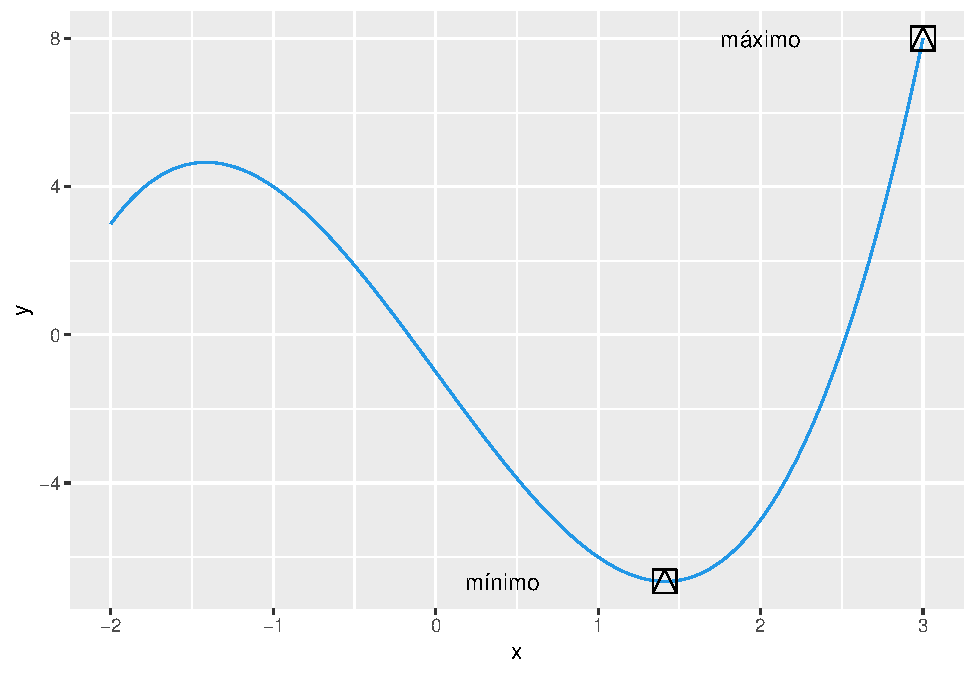
\includegraphics{gridSearch_files/figure-latex/unnamed-chunk-4-1.pdf}

\newpage
\singlespacing 
\end{document}